%%%%%%%%%%%%%%%%%%%%%%%%%%%%%%%%%%%%%%%%%
% Jacobs Landscape Poster
% LaTeX Template
% Version 1.0 (29/03/13)
%
% Created by:
% Computational Physics and Biophysics Group, Jacobs University
% https://teamwork.jacobs-university.de:8443/confluence/display/CoPandBiG/LaTeX+Poster
% 
% Further modified by:
% Nathaniel Johnston (nathaniel@njohnston.ca)
%
% This template has been downloaded from:
% http://www.LaTeXTemplates.com
%
% License:
% CC BY-NC-SA 3.0 (http://creativecommons.org/licenses/by-nc-sa/3.0/)
%
%%%%%%%%%%%%%%%%%%%%%%%%%%%%%%%%%%%%%%%%%

%----------------------------------------------------------------------------------------
%	PACKAGES AND OTHER DOCUMENT CONFIGURATIONS
%----------------------------------------------------------------------------------------

\documentclass[final]{beamer}

\usepackage[scale=1.24]{beamerposter} % Use the beamerposter package for laying out the poster

\usetheme{confposter} % Use the confposter theme supplied with this template

\setbeamercolor{block title}{fg=ngreen,bg=white} % Colors of the block titles
\setbeamercolor{block body}{fg=black,bg=white} % Colors of the body of blocks
\setbeamercolor{block alerted title}{fg=white,bg=dblue!70} % Colors of the highlighted block titles
\setbeamercolor{block alerted body}{fg=black,bg=dblue!10} % Colors of the body of highlighted blocks
% Many more colors are available for use in beamerthemeconfposter.sty

%-----------------------------------------------------------
% Define the column widths and overall poster size
% To set effective sepwid, onecolwid and twocolwid values, first choose how many columns you want and how much separation you want between columns
% In this template, the separation width chosen is 0.024 of the paper width and a 4-column layout
% onecolwid should therefore be (1-(# of columns+1)*sepwid)/# of columns e.g. (1-(4+1)*0.024)/4 = 0.22
% Set twocolwid to be (2*onecolwid)+sepwid = 0.464
% Set threecolwid to be (3*onecolwid)+2*sepwid = 0.708

\newlength{\sepwid}
\newlength{\onecolwid}
\newlength{\twocolwid}
\newlength{\threecolwid}
\setlength{\paperwidth}{48in} % A0 width: 46.8in
\setlength{\paperheight}{36in} % A0 height: 33.1in
\setlength{\sepwid}{0.024\paperwidth} % Separation width (white space) between columns
\setlength{\onecolwid}{0.22\paperwidth} % Width of one column
\setlength{\twocolwid}{0.464\paperwidth} % Width of two columns
\setlength{\threecolwid}{0.708\paperwidth} % Width of three columns
\setlength{\topmargin}{-0.5in} % Reduce the top margin size
%-----------------------------------------------------------

\usepackage{graphicx}  % Required for including images

\usepackage{booktabs} % Top and bottom rules for tables

\usepackage{exscale}

\usepackage{subfig}

%----------------------------------------------------------------------------------------
%	TITLE SECTION 
%----------------------------------------------------------------------------------------

\title{Predicting Food Inspection Outcomes in Chicago} % Poster title

\author{Luke Farewell, Jake Gober, Sam Green, Jeremy Welborn} % Author(s)

\institute{Computer Science 109a / Statistics 121a, Harvard University} % Institution(s)

% \logo{figures/SEASLogo_CMYK_Centered.png}

%----------------------------------------------------------------------------------------

\begin{document}

\addtobeamertemplate{block end}{}{\vspace*{2ex}} % White space under blocks
\addtobeamertemplate{block alerted end}{}{\vspace*{2ex}} % White space under highlighted (alert) blocks

\setlength{\belowcaptionskip}{2ex} % White space under figures
\setlength\belowdisplayshortskip{2ex} % White space under equations

\begin{frame}[t] % The whole poster is enclosed in one beamer frame

\begin{columns}[t] % The whole poster consists of three major columns, the second of which is split into two columns twice - the [t] option aligns each column's content to the top

\begin{column}{\sepwid}\end{column} % Empty spacer column

\begin{column}{\onecolwid} % The first column

%----------------------------------------------------------------------------------------
%	OBJECTIVES
%----------------------------------------------------------------------------------------

\begin{alertblock}{Objectives}

Chicago's Department of Public Health is responsible for 
inspecting 15,000 food establishments across the city. 
Our goal was to reduce the amount of time required to 
discover critical violations: 

\begin{itemize}
\item Aggregate and clean useful data sources.
\item Build models for probabilities of failure.
\item Optimize inspection efficiency and social
cost of undiscovered health risks.
\end{itemize}

\end{alertblock}

%----------------------------------------------------------------------------------------
%	INTRODUCTION
%----------------------------------------------------------------------------------------

\begin{block}{Data: Sources and Cleaning}

% \setlength\tabcolsep{1.2in}
\def\arraystretch{1.5}
\begin{tabular}{|c| c|}
\hline
\textbf{Food Inspections} & \textbf{Business Activities} \\ \hline
\textbf{Weather} & \textbf{Crime Reports} \\ \hline
\textbf{Sanitation Complaints} & \textbf{Business Location}\\ \hline
\end{tabular}\vspace{0.2in.}
Sources: City of Chicago Open Data Portal, NOAA. 

\begin{enumerate}
    \item Pair inspections with business information.
    \item Process past inspection text to build history.
    \item Bucket spatial data with a grid (see visualizations).
\end{enumerate}

\end{block}

\vspace{-1in.}
\begin{block}{Exploration (I)}
\begin{figure}[H]
  \centering
    \subfloat{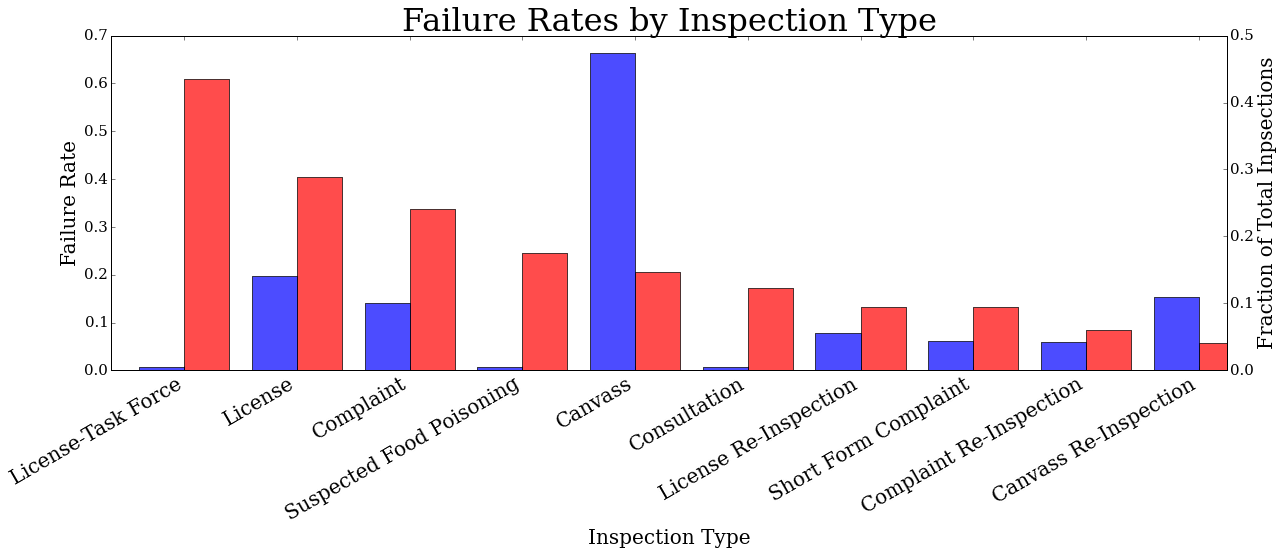
\includegraphics[width = \linewidth]{figures/exploration/exp_1_top.png}}

    \subfloat{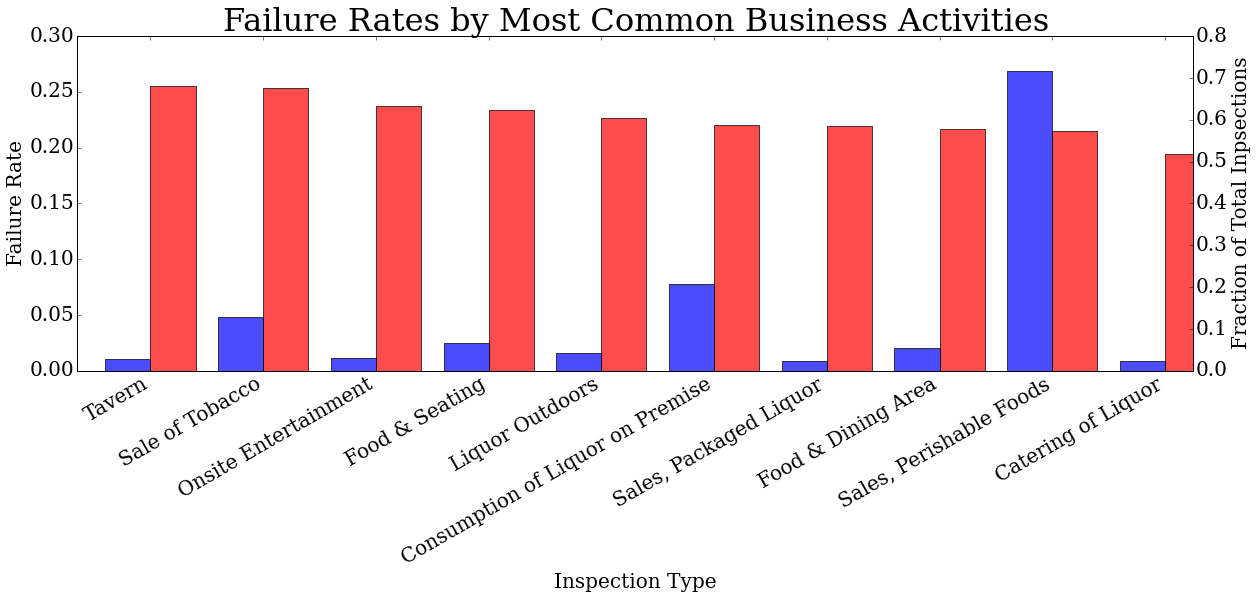
\includegraphics[width = \linewidth]{figures/exploration/exp_1_bot.png}}
  \caption{Inspection Results by Feature}
\end{figure}
\end{block}


%----------------------------------------------------------------------------------------

\end{column} % End of the first column

\begin{column}{\sepwid}\end{column} % Empty spacer column

\begin{column}{\twocolwid} % Begin a column which is two columns wide (column 2)

\begin{columns}[t, totalwidth=\twocolwid]

\begin{column}{\onecolwid}\vspace{-.6in.}
\begin{block}{Results (I): Unsuccessful Models}

\begin{figure}
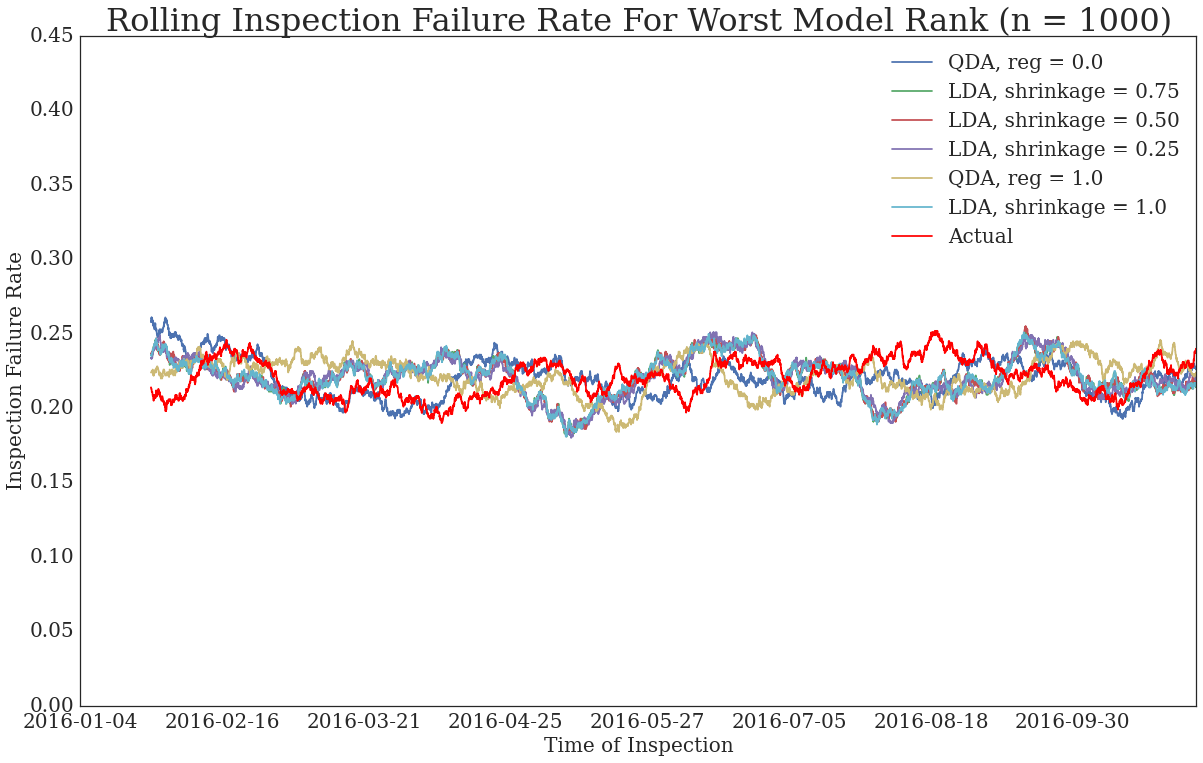
\includegraphics[width=\linewidth]{figures/exploration/rolling_failure_bad.png}
\caption{Rolling Failure Rate, Poorly Performing Models}
\end{figure}
\end{block}

\end{column}

\begin{column}{\onecolwid}\vspace{-.6in.}
\begin{block}{Results (II): Successful Models}
\begin{figure}
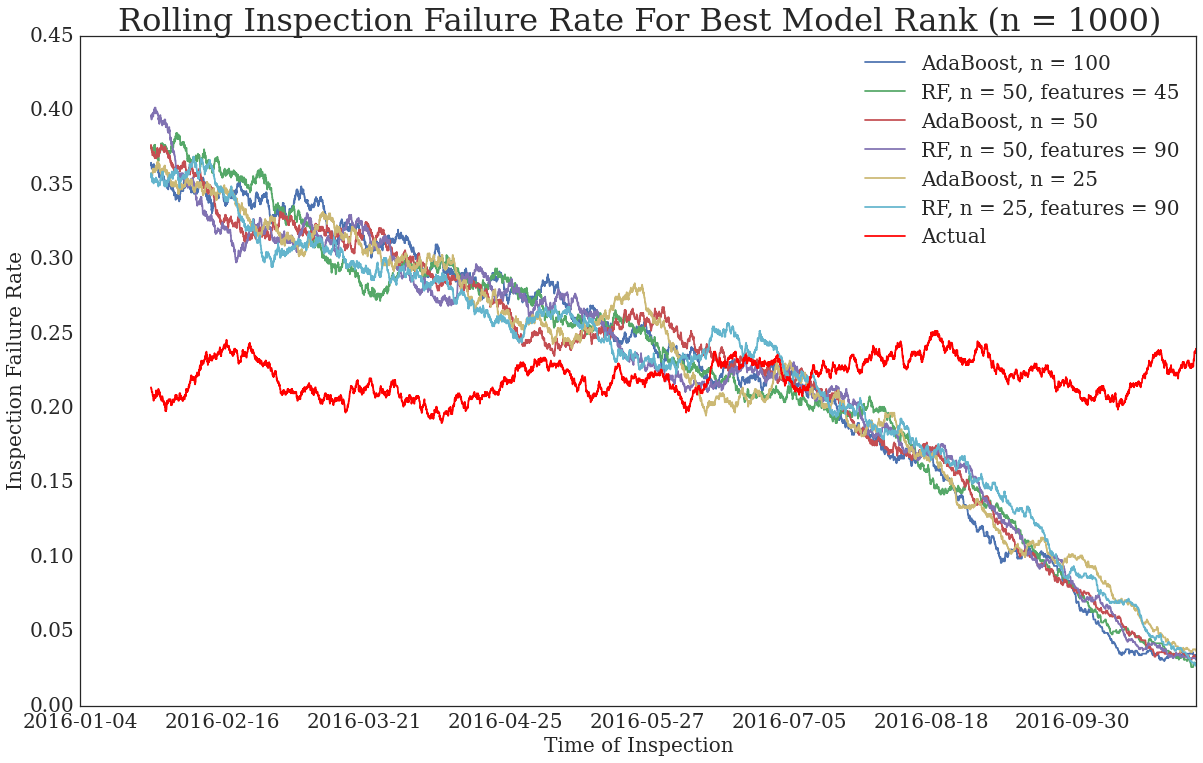
\includegraphics[width=\linewidth]{figures/exploration/rolling_failure_good.png}
\caption{Rolling Failure Rate, Well Performing Models}
\end{figure}
\end{block}
\end{column}
\end{columns}

\vspace{-1in}
\begin{columns}[t, totalwidth=\twocolwid]
\begin{column}{\onecolwid}
\begin{alertblock}{Model Scoring: Log Loss}

To measure \textit{rank accuracy} and match the 
recommendation setting, 
we selected \textbf{log loss} as our scoring function.

\begin{equation}
-\frac{1}{n} \sum_{1}^{n} [y_i \log(p_i)-(1-y_i)\log(1-p_i)]
\end{equation}
for $n$ observations, where the $i$th observation is of correct class $y_i \in \{0,1\}$ 
which our model assigns probability $p_i$.

\end{alertblock}
\end{column}

\begin{column}{\onecolwid}
\begin{alertblock}{Model Selection: Rank Quality}

To choose between models, we treated test data
as undated possible inspections and select the model
that minimizes

\begin{equation}
\frac{1}{n} \sum_i^n \mathbf{1}_{y_i = 1} * n_i^{\text{days\_to\_discover}}
\end{equation}

because the goal is to catch failures as early as 
possible. This quantity is the average days until true failures are discovered.

\end{alertblock}
\end{column}
\end{columns}

\begin{column}{\twocolwid}\vspace{-.6in} % The first column within column 2 (column 2.1)

%----------------------------------------------------------------------------------------
%   Data Collection
%----------------------------------------------------------------------------------------

\begin{block}{Exploration (III): Spatial Predictors \& Neighborhood Dynamics}

\begin{figure}
% \subfigure[] 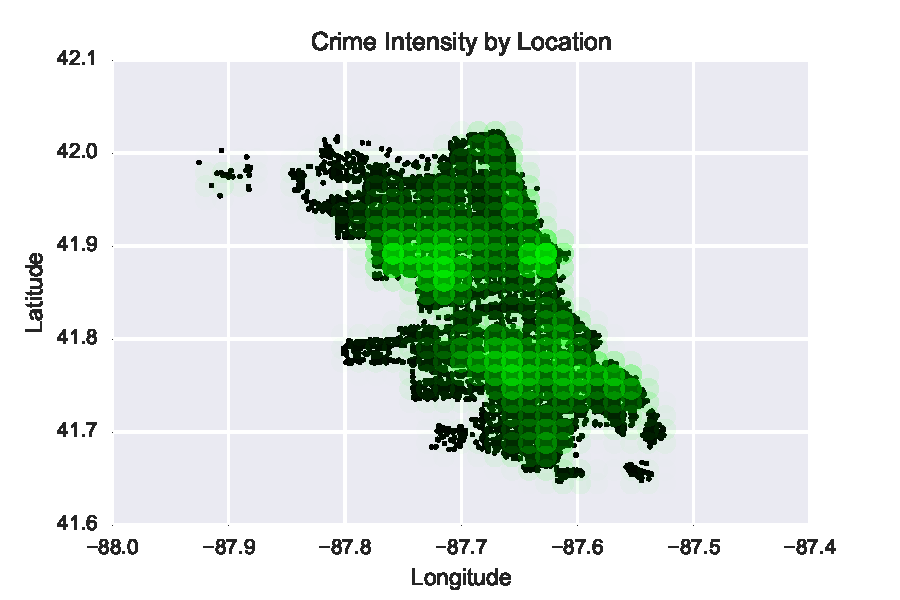
\includegraphics[width=0.8\linewidth]{figures/crime.png}
%
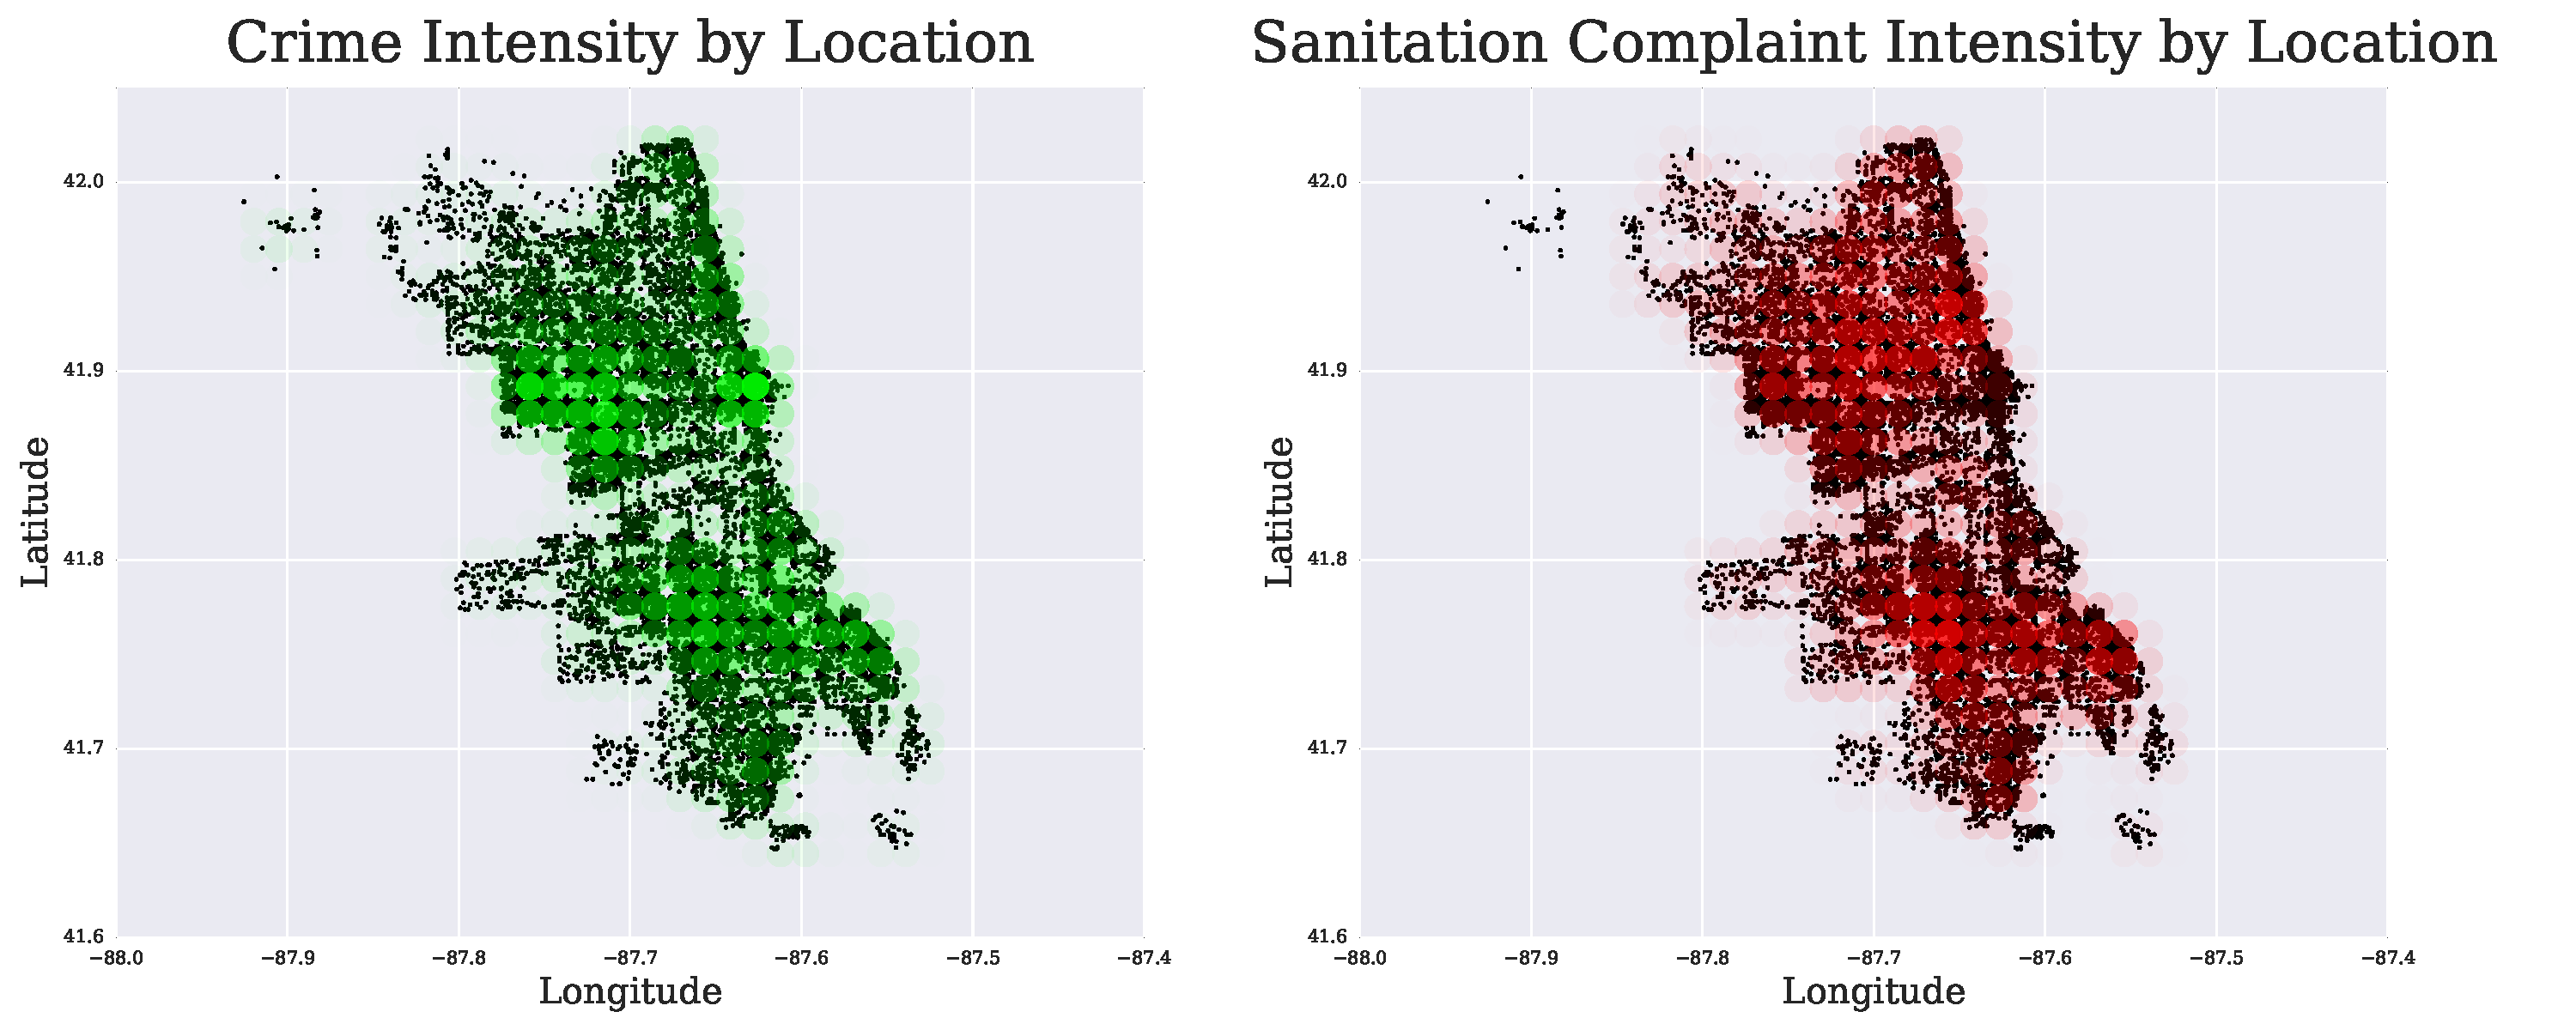
\includegraphics[width=\linewidth]{figures/both.pdf}
\caption{Crime (left) and Sanitation Complaint (Right) by Location. Darker shades represent 
a larger fraction of observations. }
\end{figure}

\end{block}
\end{column}

\end{column} % End of the second column

\begin{column}{\sepwid}\end{column} % Empty spacer column

\begin{column}{\onecolwid} % The third column

%----------------------------------------------------------------------------------------
%	CONCLUSION
%----------------------------------------------------------------------------------------

\begin{block}{Results (III)}

Based on our cross-validition process, 
AdaBoost was selected as the optimal
model in this setting, as shown
below in the barchart displaying
the selection statistic:  

\begin{figure}
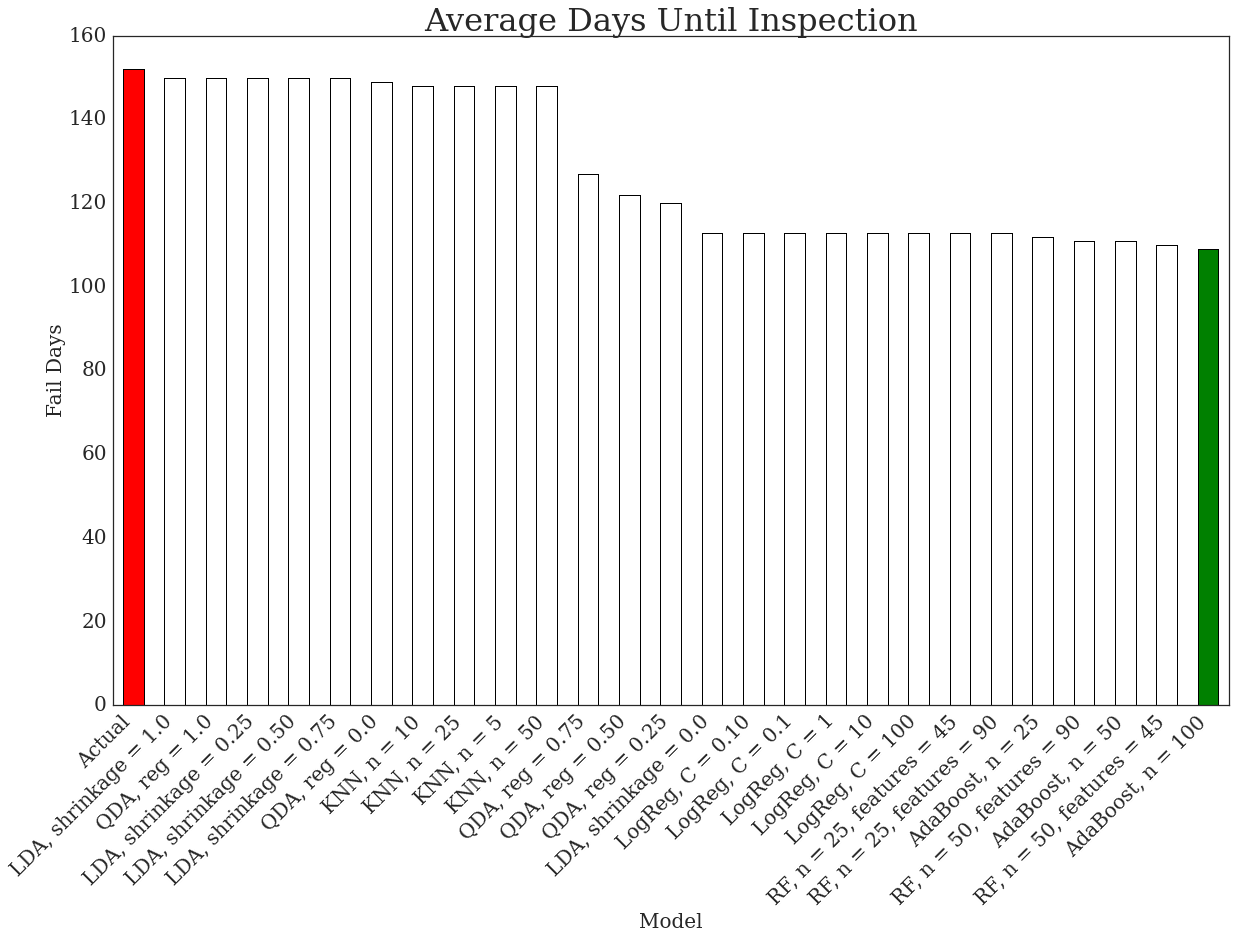
\includegraphics[width=\linewidth]{figures/exploration/bar_result.png}
\caption{Average days to discovery for failing businesses.}
\end{figure}

A boosted Random Forest model is intuitive in this
setting, considering that several predictors were
highly non-linear in the response. All 
of the best performing models are bagged or 
boosted decision tree ensemble methods. 

\end{block}

\vspace{-1in.}
\begin{block}{Next Steps}

Currently the model ranks all possible inspections
in the testing data, but in practice,
it would be ranking inspections of all possible
businesses and itself determining what inspections
actually take place. The model also does not account for the 
gradual appearance of complaints over time. \\ 

\vspace{.4in}

As a result, the frequency with which the model
is reset needs to be tuned, to set the $d$ days
worth of inspections generated by each ranking.
\end{block}


%----------------------------------------------------------------------------------------
%	ACKNOWLEDGEMENTS
%----------------------------------------------------------------------------------------

% \setbeamercolor{block title}{fg=red,bg=white} % Change the block title color

% \begin{block}{Acknowledgements}

% \small{\rmfamily{Nam mollis tristique neque eu luctus. Suspendisse rutrum congue nisi sed convallis. Aenean id neque dolor. Pellentesque habitant morbi tristique senectus et netus et malesuada fames ac turpis egestas.}} \\

% \end{block}

%----------------------------------------------------------------------------------------
%	CONTACT INFORMATION
%----------------------------------------------------------------------------------------

\setbeamercolor{block alerted title}{fg=black,bg=norange} % Change the alert block title colors
\setbeamercolor{block alerted body}{fg=black,bg=white} % Change the alert block body colors

\begin{alertblock}{Contact Information}

\begin{itemize}
\item Web: \href{https://fggw.github.io/foodinspections/}{fggw.github.io/foodinspections/}
\item Code: \href{http://github.com/fggw/foodinspections}{github.com/fggw/foodinspections/}
\item Contact: \{lfarewell, jgober, samuelgreen, jeremywelborn\}@college.harvard.edu
\end{itemize}

\end{alertblock}

%----------------------------------------------------------------------------------------
%   REFERENCES
% %----------------------------------------------------------------------------------------

% \begin{block}{References}
% \begin{itemize}
%     \item \href{https://chicago.github.io/food-inspections-evaluation/}{https://chicago.github.io/food-inspections-evaluation/}
% \end{itemize}
% \end{block}

%----------------------------------------------------------------------------------------

\end{column} % End of the third column

\end{columns} % End of all the columns in the poster

\end{frame} % End of the enclosing frame

\end{document}
